\subsection{二维图像语义分割}

% \subsubsection{简介}

\par 对二维图像进行语义分割属于全景分割(Panoptic Segmentation,如图\ref{fig:panopticsegmentation})\cite{panopticsegmentation}的一部分,是计算机视觉领域的一项重要任务,
旨在将输入的二维图像中每个像素分配给特定的语义类别,如人、车、树等。这意味着对图像进行像素级别的分类和分割,使每个像素都被标记为属于图像中的哪个类别。
\begin{figure}[htbp]
	\centering
	\subfigure[RGB图像]{
		\begin{minipage}[t]{0.45\linewidth}
			\centering
			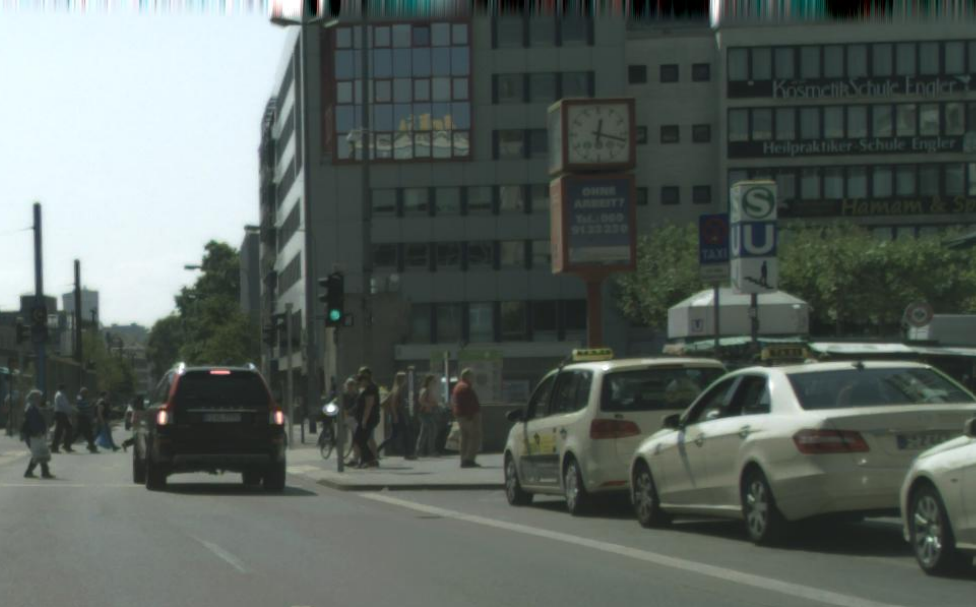
\includegraphics[height=4cm,keepaspectratio]{figures/panoptic_seg_1.png}
		\end{minipage}
	}
	\subfigure[语义图像]{
		\begin{minipage}[t]{0.45\linewidth}
			\centering
			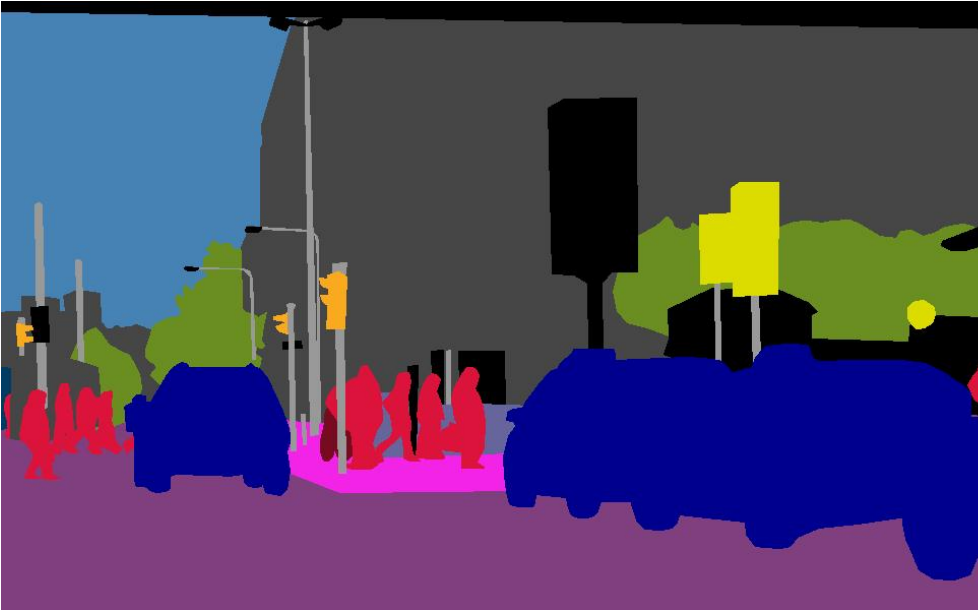
\includegraphics[height=4cm,keepaspectratio]{figures/panoptic_seg_2.png}
		\end{minipage}
	}

	\subfigure[实例图像]{
		\begin{minipage}[t]{0.45\linewidth}
			\centering
			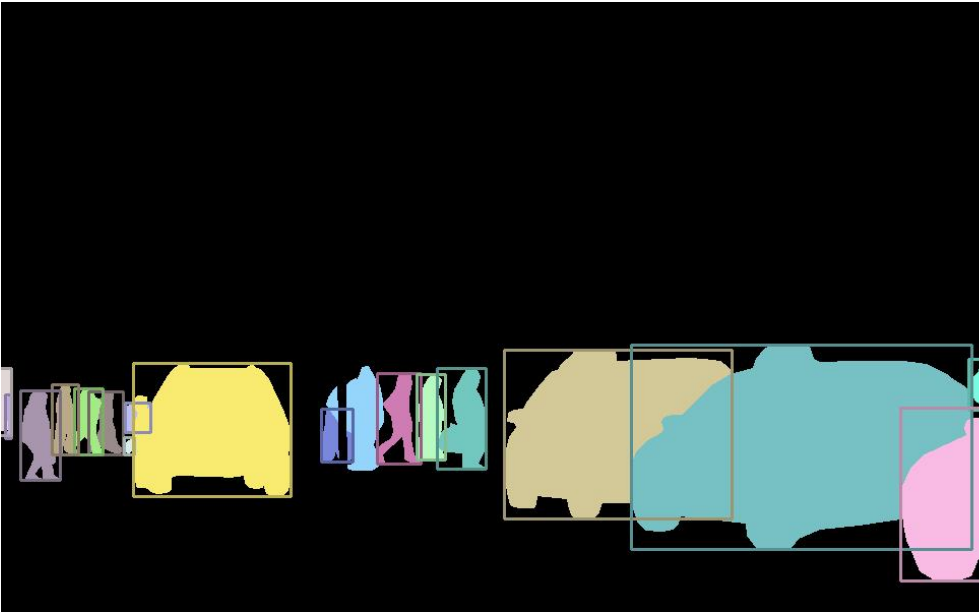
\includegraphics[height=4cm,keepaspectratio]{figures/panoptic_seg_3.png}
		\end{minipage}
	}
	\subfigure[全景图像]{
		\begin{minipage}[t]{0.45\linewidth}
			\centering
			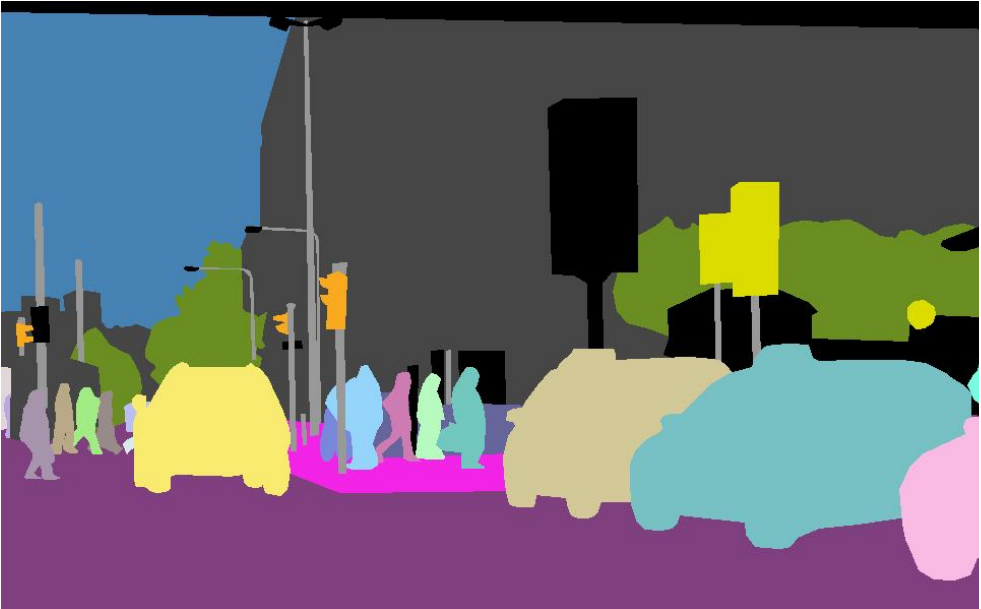
\includegraphics[height=4cm,keepaspectratio]{figures/panoptic_seg_4.png}
		\end{minipage}
	}
	\caption{二维图像全景分割}
	\label{fig:panopticsegmentation}
	\note{注:对于给定的RGB图像(a),(b)为语义分割,每个像素对应一个类别。(c)为实例分割,每个像素对应一个实例。(d)为全景分割。}
\end{figure}
语义分割对于自动驾驶、物体识别、场景理解等应用具有重要意义,可以为计算机系统提供更深入的关于图像内容的理解,为各种应用提供更准确和有用的信息。

% \subsubsection{研究现状}
\par 语义分割自从被提出以来,已经取得了显著的进展\cite{pascal,sift_flow,textonboost}。以下是截止2023年5月的一些研究现状:

\paragraph{SegNet}
\par 2015年,Vijay Badrinarayanan等人提出了SegNet\cite{segnet},这是一个基于编码器-解码器架构的深度学习模型。
SegNet的编码器网络对图像进行下采样以提取特征,然后解码器网络将这些特征图上采样回原始图像的大小,以进行像素级的分类。

\paragraph{Deeplab系列}
\par Deeplab\cite{deeplab}是一种高效的深度学习模型,它在语义分割任务中达到了很高的精度。Deeplab的主要创新是使用了空洞卷积(Dilated
Convolution)和条件随机场(Conditional Random Fields,CRF)。
空洞卷积可以在不增加计算复杂度的情况下增大感受野,而条件随机场可以改善分割结果的细节部分。后续的Deeplabv2\cite{deeplab2}、Deeplabv3
和 Deeplabv3+\cite{deeplab3plus}进一步提升了性能, 其中Deeplabv3引入了空洞空间金字塔池化模块(Atrous
Spatial Pyramid Pooling,ASPP)模块以捕获多尺度信息,Deeplabv3+
则加入了编码器-解码器结构,提升了分割的精度,如图\ref{fig:Deeplabv3+}\cite{deeplab3plus}所示。

\begin{figure}[htb]
	\centering
	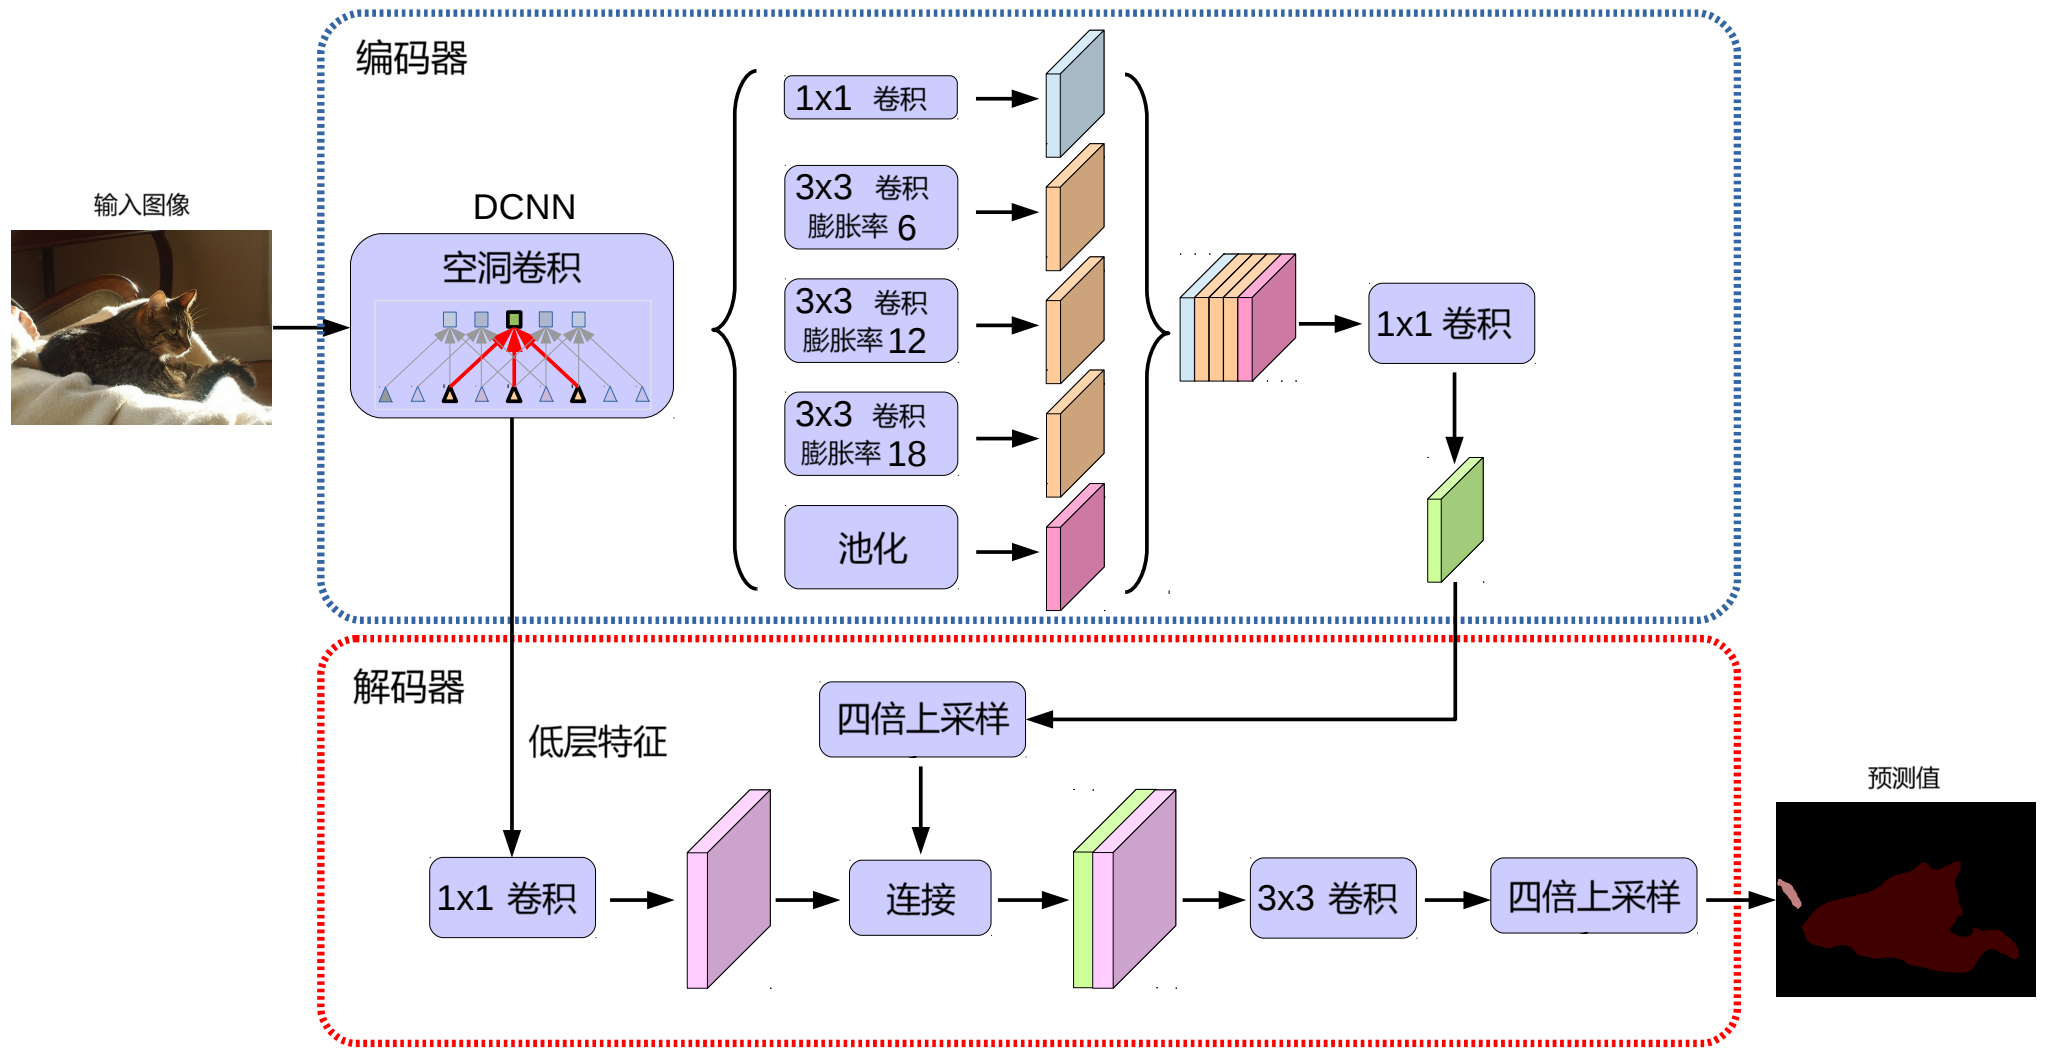
\includegraphics[width=0.9\textwidth]{figures/deeplab3_endecoder.png}
	\caption{Deeplabv3+的编码器-解码器结构}
	\label{fig:Deeplabv3+}
	\note{注:DeepLabv3+ 通过采用编码器-解码器结构扩展 DeepLabv3。其中,编码器通过在多个尺度应用空洞卷积实现编码多尺度上下文信息,而解码器则沿对象边界细化分割结果。}
\end{figure}

\paragraph{SAM}
\par SAM(Segment Anything Model)\cite{segment_anything}是由 Meta AI Research 开发,于 2023
年4月首次推出的一个模型,可用于分割图像中的任何对象。
该模型在图\ref{fig:sa-1b}\cite{segment_anything}所示的1100万张图像和11亿个掩码的大规模数据集SA-1B上进行训练,无需对新对象或图像进行额外的训练即可进行分割,生成高质量的分割掩码。
尽管 SAM 仍在开发过程中,但是它已经在各种场景中展示出巨大的应用潜力,有可能彻底改变我们与计算机和周围世界的互动方式。

\begin{figure}[htb]
	\centering
	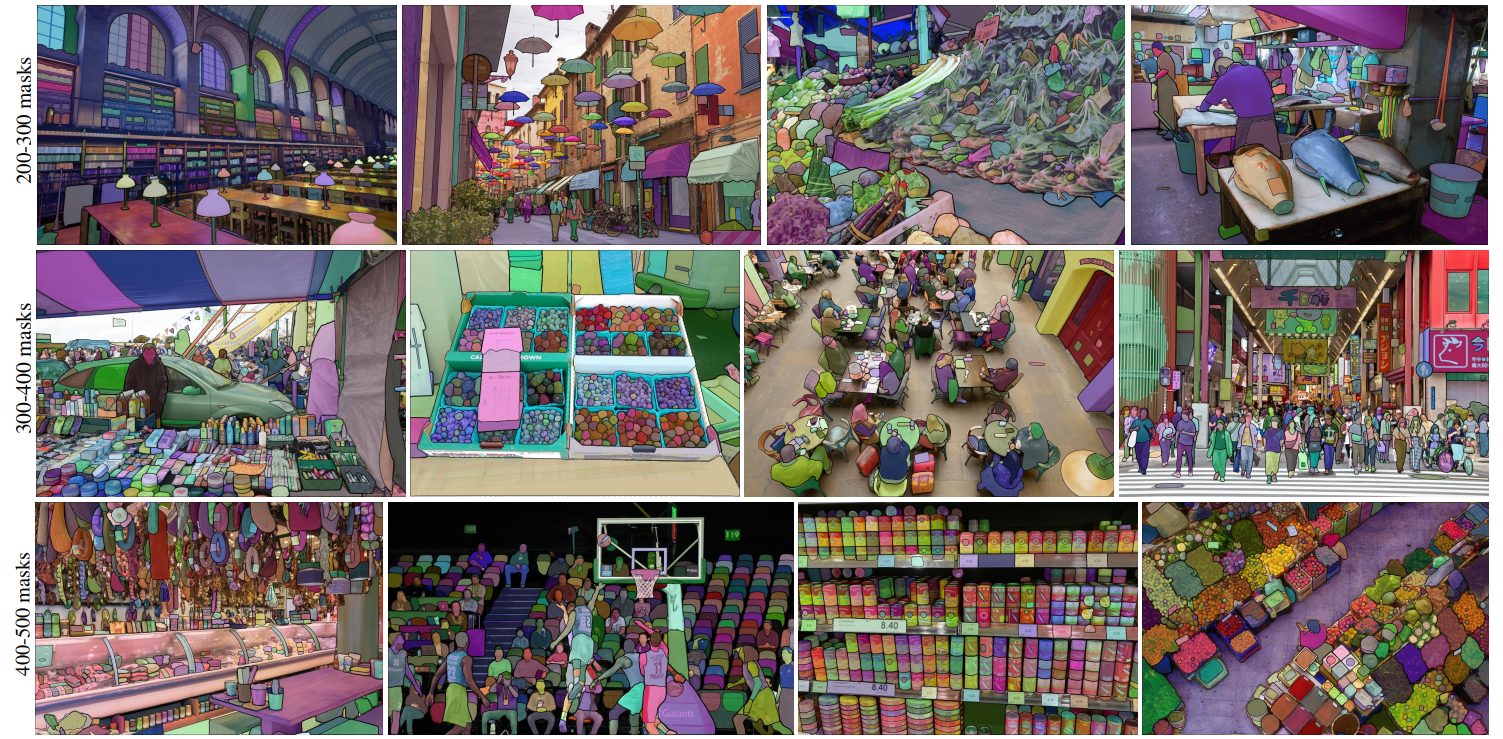
\includegraphics[width=0.9\textwidth]{figures/sam_result.png}
	\caption{SA-1B数据集示例图}
	\label{fig:sa-1b}
	\note{注:SA-1B数据集包含了1100万高质量、多样化的图片及11亿个精确分割蒙版示例。}
\end{figure}

\par 尽管语义分割已经取得了很大的进展,但它仍然面临着处理多尺度问题、减小计算复杂度和提高分割精度等挑战。
为了解决这些问题,未来的研究将主要集中在三个方向:
首先是端到端的训练方法\cite{pspnet,deeplab3plus}。这种方法可以一次性完成整个任务,提高了效率并且能够避免不一致的结果;
其次,随着计算机视觉技术的发展,语义分割被期待在嵌入式设备和实时应用中发挥更大的作用,这需要提高分割算法的效率和速度;
最后,多模态语义分割,即整合多种类型的输入数据,如雷达、激光雷达(LiDAR)或声音,将有助于提供更准确和更鲁棒的结果\cite{SceneParsing,CascadedPyramidNetwork}。